\documentclass[12pt]{article}

\usepackage{comptype}

\title{%%
Lista de Computação para Arquitetura\\
{\normalsize LAMO / FAU / UFRJ}
}

\author{%%
Pedro Maciel Xavier \\ 
\texttt{pedromxavier@poli.ufrj.br}
}

\date{}

\begin{document}
	\maketitle
	
	\tableofcontents
	
	\cc
	
	\pagebreak
	
	
	\section{Aula I - Tipos, Variáveis e Funções \\ (\stmt{def}, \stmt{return})}
	
	\problem[0]{As notas musicais}
	
	Cada nota musical corresponde a uma frequência distinta (em Hz). Tomando o lá central (A4) como referência, em 440Hz, podemos calcular a frequência das outras notas com base na distância relativa a essa nota.
	$$f(n) = 440 \times 2^{(n/12)}$$
	Na tabela abaixo, vemos as notas musicais, seus símbolos, e a distância em semitons\footnote{Um Tom equivale a dois Semitons.} para o lá central (A4).
	
	\begin{center}
		\begin{tabular}{|l|c c c c c c c c c c c c|}
			\hline
			Símbolo &  & F3 & G3 & A4 & B4 & C4 & D4 & E4 & F4 & G4 & A5 & \\
			Nome & ... & fá & sol & lá & si & dó & ré & mi & fá & sol & lá & ... \\
			Semitons &  & -4 & -2 & 0 & 2 & 3 & 5 & 7 & 8 & 10 & 12 & \\
			\hline
		\end{tabular}
	\end{center}

	Você pode notar que a cada 12 semitons, a nota se repete com o dobro da frequência. Chamamos este intervalo entre notas de oitava. Na notação acima, a cada letra indica uma nota diferente, enquanto o número diz a oitava em que ela se encontra.\\
	
	\quest Faça uma função \texttt{f(n)} que retorne a frequência em Hertz de uma nota que se encontra a \texttt{n} semitons de distância do lá central. Arredonde o resultado para o número inteiro mais próximo usando as funções \type{round} e \type{int}.\\
	
	\example 
	\begin{lstlisting}
>>> f(0)
440
>>> f(2)
494
>>> f(3)
523
>>> f(12)
880
	\end{lstlisting}
	
	\vfill
	
	\pagebreak
	
	\problem[0]{Coordenadas polares}
	
	Estamos acostumados a pensar em coordenadas cartesianas na hora de descrever a geometria de um determinado objeto. No entanto, o sistema de coordenadas deve ser escolhido conforme o cenário em que se está trabalhando.
	
	\begin{figure}[H]
	\centering
	\resizebox{200pt}{!}{%
	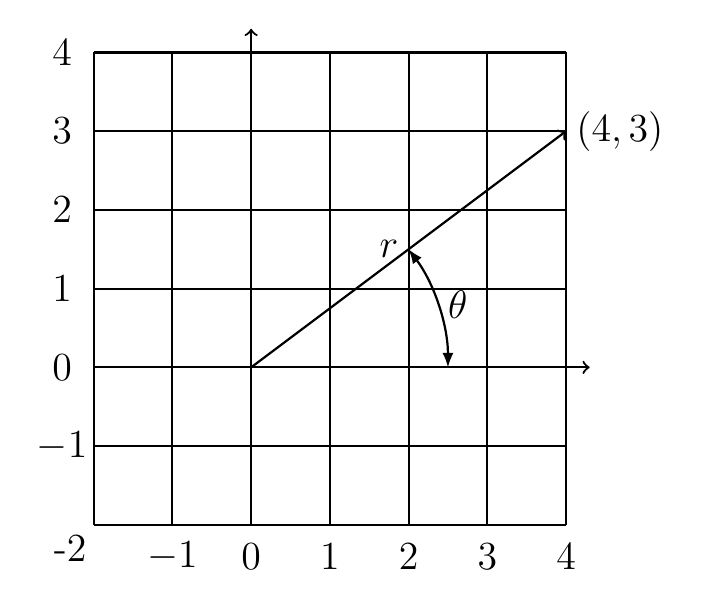
\begin{tikzpicture}[thick,font=\Large]
		\draw[step=1.0,black,thick] (-2,-2) grid (4, 4);
		\foreach \i in {-1, ..., 4} {
			\node[align=left] at (\i, -2.4) {$\i$};
			\node[align=left] at (-2.4, \i) {$\i$};
		}
		\node at (-2.3, -2.3) {-2};
		%% Axis
		\draw[->] (4, 0) -- (4.3, 0);
		\draw[->] (0, 4) -- (0, 4.3);
		%% else
		\draw[thick, ->] (0, 0) -- (4, 3) node [midway, left] {$r$} node [right] {$(4, 3)$};
		\draw[latex-latex]  (0:2.5) arc (0:36.87:2.5) node[midway, right]{$\theta$};
	\end{tikzpicture}
	}
	\caption{Coordenadas cartesianas e polares.}
\end{figure}
	
	O ponto $(4, 3)$, quando escrito em coordenadas polares, nos dá:
	\begin{align*}
	r &= \sqrt{4^2 + 3^2} = \sqrt{16 + 9} = \sqrt{25} = 5\\
	\theta &= \arctan\frac{3}{4} = 0.6435 \text{ rad} \approx 36.87^{\circ}
	\end{align*}
	
	\quest Construa duas funções: \texttt{polar(x, y)} levará um ponto em coordenadas cartesianas $(x, y)$ para a forma polar $(r, \theta)$ e \texttt{cart(r, theta)}, que fará o caminho contrário.\\
	
	\clue O módulo \texttt{math} contém as funções trigonométricas \texttt{math.sin}, \texttt{math.cos} e \texttt{math.tan}, assim como as inversas \texttt{math.asin}, \texttt{math.acos} e \texttt{math.atan}. Para calcula a raiz quadrada, você pode usar a função \texttt{math.sqrt}.\\
	
	\example
	\begin{lstlisting}
>>> import math
>>> polar(-1, 0)
(1.0, 3.141592653589793)
>>> cart(2, math.pi)
(-2.0, 0.0)
	\end{lstlisting}
	
	\pagebreak
	
	\problem[0]{Funções}
	
	\pagebreak
	
	\section{Aula II - Condicionais \\(\stmt{if}, \stmt{elif}, \stmt{else})}
	
	\problem[0]{Dentro do círculo}
	
	O círculo unitário é aquele que tem raio $1$ e se encontra centrado na origem $(0, 0)$ do plano cartesiano.
	
	\begin{figure}[H]
	\centering
	\resizebox{200pt}{!}{%
	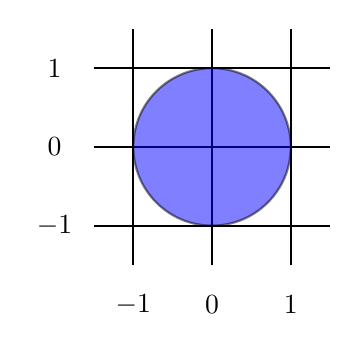
\begin{tikzpicture}[thick]
		\draw[step=1.0,black,thick] (-1.5,-1.5) grid (1.5, 1.5);
		\foreach \i in {-1, ..., 1} {
			\node[align=left] at (\i, -2) {$\i$};
			\node[align=left] at (-2, \i) {$\i$};
		}
		\draw[fill=blue, semitransparent] (0,0) circle[radius=1];
	\end{tikzpicture}
	}
	\caption{Círculo Unitário}
\end{figure}
	
	\quest Faça uma função que diga se um ponto $(x, y)$ se encontra dentro ou fora do círculo unitário, retornando \stmt{True} ou \stmt{False} respectivamente.\\
	
	\example
	\begin{lstlisting}
>>> dentro(1, 1)
False
>>> dentro(0, 0)
True
>>> dentro(1, 0)
True
>>> dentro(0.5, 0.5)
True
	\end{lstlisting}
	
	\pagebreak
	
	\problem[0]{Intersecção de Retângulos}
	
	Uma maneira simples de representar retângulos em um computador é através de um par de pontos, onde cada ponto é um par ordenado $(x, y)$. Por convenção, o primeiro ponto indica o canto superior esquerdo do retângulo; e o segundo, o canto inferior direito.\\
	
	\begin{figure}[H]
	\centering
	\begin{tikzpicture}
	\draw[draw=black] (11.1,5.5) rectangle ++(0.3,0.3);
	\end{tikzpicture}
\end{figure}
	
	Assim, o retângulo \textcolor{blue}{\textbf{azul}} pode ser descrito pelos pares $(1, 4)$ e $(5, 2)$, enquanto o retângulo \textcolor{red}{\textbf{vermelho}} é dado pelos pontos $(3, 3)$ e $(6, 1)$. A intersecção entre os dois é justamente a área \textcolor{indigo}{\textbf{lilás}} que se encontra entre os pontos $(3, 3)$ e $(5, 2)$. \\
	
	\quest Fazer uma função que, dados dois retângulos, retorna a intersecção entre eles, ou seja, um outro retângulo ou \stmt{None}, caso não haja sobreposição.\\
	
	\example
	\begin{lstlisting}
>>> A = (1, 4, 5, 2)
>>> B = (3, 3, 6, 1)
>>> C = intersec(A, B)
>>> print(C)
(3, 3, 5, 2)
	\end{lstlisting}
	
	\pagebreak
	
	\problem[0]{Anos bissextos}
	
	A humanidade sempre teve problemas com a contagem dos anos, uma vez que estes duram 365,24 dias. O calendário Juliano, que vigorou de 45 a.C. até 1582 d.C., introduziu o uso dos anos bissextos acrescentou um dia a cada 3 anos. O erro só foi percebido décadas depois e o acréscimo foi abandonado. Isso fez com que se acumulasse um erro de cerca de 10 dias até o momento da transição para o calendário Gregoriano. Por conta disso, os dias entre 4 e 15 de outubro de 1582 simplesmente não existiram.\\
	
	Com este novo calendário foi definida a nova regra para o cálculo dos anos bissextos:
	
	\begin{itemize}
		\item De 4 em 4 anos é ano bissexto.
		\item De 100 em 100 anos não é ano bissexto.
		\item De 400 em 400 anos é ano bissexto.
		\item Prevalecem as últimas regras sobre as primeiras.
	\end{itemize}
	
	\quest Sabendo que o ano 2000 foi bissexto, crie uma função que, dado um ano, informe se ele é bissexto ou não, retornando \stmt{True} ou \stmt{False}, respectivamente.\\
	
	\example
	\begin{lstlisting}
>>> bissexto(2000)
True
>>> bissexto(2100)
False
>>> bissexto(2104)
True
	\end{lstlisting}
	
	\pagebreak
	
	\problem[0]{Meia-entrada}
	
	A Lei Federal nº 12933/2013, também conhecida como Lei da Meia-Entrada, garante o benefício do pagamento de Meia-Entrada para estudantes, pessoas com deficiência e jovens, de baixa renda, com idade entre 15 e 29 anos. Já a Lei Federal nº 10741/2003, mais conhecida como Estatuto do Idoso, as pessoas com idade igual ou superior a 60 anos tem direito à Meia-Entrada para eventos artísticos e de lazer. Aqui no estado do Rio de Janeiro, contamos ainda com a Lei Estadual RJ n° 3.364/00, que garante o benefício a todos os menores de 21 anos.\\
	
	\quest Escreva a função \texttt{meia\_entrada} que receba os parâmetros \texttt{idade} (\type{int}), \texttt{estudante} (\type{bool}), \texttt{deficiencia} (\type{bool}), \texttt{baixa\_renda} (\type{bool}) e informe com \stmt{True} ou \stmt{False} se a pessoa tem direito ao desconto.\\
	
	\example
	\begin{lstlisting}
>>> meia_entrada(60, False, False, False)
True
>>> meia_entrada(30, True, False False)
False
>>> meia_entrada(20, False, False, False)
True
	\end{lstlisting}
	
	\pagebreak
	
	\section{Aula III - Listas e Loops \\(\stmt{while}, \stmt{for})}
	
	\problem[0]{Sequência de \emph{Collatz}}
	
	A sequência de \emph{Collatz} é obtida aplicando sucessivamente a função
	{\large
		\begin{align*}
		f(n) = \begin{cases}
		3n + 1, &\text{ se } n \text{ for ímpar}\\
		n \div 2, &\text{ se } n \text{ for par}
		\end{cases}
		\end{align*}
	}
	Por exemplo, começamos com $n = 26$. Após sucessivas aplicações temos:
	$$26 \to 13 \to 40 \to 20 \to 10 \to 5 \to 16 \to 8 \to 4 \to 2 \to 1$$
	Isso nos dá uma sequência com $11$ números. $40$ é maior que $26$, mas sua sequência só teria $9$ números.\\
	\\
	Ainda não se sabe se todos os números induzem uma sequência que termina em $1$. No entanto, até agora não foi encontrado um número sequer em que isso não tenha acontecido!\\
	\\
	\quest Faça uma função que calcule o comprimento da sequência gerada a partir de um número natural $n$ qualquer.\\
	
	\example
	\begin{lstlisting}
>>> collatz(26)
11
>>> collatz(40)
9
>>> collatz(1)
1
	\end{lstlisting}
	
	\pagebreak
	
	\problem[0]{Crivo}
	
	O Eratóstenes foi um cara que viveu em 200 a.C., inventou um crivo e calculou a curvatura da terra.
	\vspace{-10pt}
	\figura[width=100pt]{eratostenes.png}{Eratóstenes de Cirene}
	\vspace{-30pt}
	Um \textbf{crivo} é uma forma de saber quem são os números primos até um determinado limite $\mb{N}$. O Crivo de Eratóstenes funciona de forma bem simples:
	
	\begin{enumerate}
		\item Escrevemos em uma tabela todos os números de 0 até $\mb{N}$.

		\item Riscamos o 0 e o 1 e andamos para o 2.

		\item Se um número não estiver riscado, riscamos todos os múltiplos deste, menos o próprio.
		
		\item Andamos para o próximo número e repetimos a etapa anterior (3).		
	\end{enumerate}
	
	Uma maneira interessante de fazer isso é criando uma lista \texttt{L} de tamanho $\mb{N} + 1$, ou seja, cujos índices vão de 0 até $\mb{N}$. Nessa lista, a princípio, supomos que todos os números são primos, então todas as suas entradas serão \stmt{True}. Riscar um número significa transformar uma entrada em \stmt{False}\\
	
	\quest Implemente o crivo de Eratóstenes, retornando uma lista com os números primos entre 0 e $\mb{N}$.\\
	
	\example
	\begin{lstlisting}
>>> crivo(10)
[2, 3, 5, 7]
>>> crivo(20)
[2, 3, 5, 7, 11, 13, 17, 19]
	\end{lstlisting}
	
	\pagebreak
	
	\problem[0]{Loops}

	\pagebreak	
\end{document}